% These are the lecture notes for my CSCI360 course SPRING 2017
% at John Jay College of Criminal Justice. They are based largely on
% Schneier's Applied Cryptography.

% Feel free to edit these slides and use them for your own courses.
% HOWEVER DO NOT REMOVE THESE LINES!
% Email me at: awood [at] jjay.cuny.edu
% or at: awood [at] gradcenter.cuny.edu


\documentclass{beamer}

\usepackage{tikz}
\usetikzlibrary{calc}

\usepackage{forest}
\usepackage{verbatim}
\usepackage{color}
\usepackage{amsmath}
\usepackage{graphicx}
\usepackage{caption}



\setbeamertemplate{footline}[frame number]
\setbeamertemplate{navigation symbols}{} 

\newtheorem{thm}{Theorem}[section]
\newtheorem{lem}{Lemma}
\newtheorem{cl}{Claim}
\newtheorem{cor}{Corollary}[section]
\newtheorem{conj}{Conjecture}
\newtheorem{quest}{Question}
\newtheorem{defn}{Definition}[section]
\newtheorem{obs}{Observation}[section]
\newtheorem{exam}{Example}

\newcommand{\im}{\operatorname{im}}
\newcommand{\id}{\operatorname{id}}
\newcommand{\interior}{\operatorname{int}}
\newcommand{\bdry}{\operatorname{bdry}}
\newcommand{\<}{\langle}
\renewcommand{\>}{\rangle}
\newcommand{\Gab}{(G_\phi)^{ab}} 
\newcommand{\phibar}{\bar{\phi}}
\newcommand{\Z}{\mathbb{Z}}
\newcommand{\N}{\mathbb{N}}
\newcommand{\Q}{\mathbb{Q}}
\newcommand{\R}{\mathbb{R}}
\newcommand{\C}{\mathbb{C}}
\newcommand{\A}{\mathcal{A}}
\newcommand{\OO}{\mathcal{O}}
\newcommand{\UU}{\mathcal{U}}
\newcommand{\power}{2^{\{P_1, \cdots , P_n\}}}
\newcommand{\bp}{\begin{problem}}
\newcommand{\ep}{\end{problem}}
\newcommand{\ba}{\begin{answer}}
\newcommand{\ea}{\end{answer}}
\newcommand{\ds}{\displaystyle}
\newcommand{\ben}{\renewcommand{\theenumi}{\alph{enumi}}
\renewcommand{\labelenumi}{(\theenumi)}\begin{enumerate}}
\newcommand{\een}{\end{enumerate}}
\newcommand{\Hess}{\operatorname{Hessian}}
\newcommand{\Aut}{\mathrm{Aut}}
\newcommand{\Inn}{\mathrm{Inn}}
\newcommand{\Out}{\mathrm{Out}}
\newcommand{\End}{\mathrm{End}}


\mode<presentation>
{
%  \usetheme{default}
  \setbeamercovered{invisible}
}


\usepackage[english]{babel}
\usepackage[latin1]{inputenc}
\usepackage{times}
\usepackage[T1]{fontenc}
\usepackage{stmaryrd}

%\usetheme{default}
%\usetheme{AnnArbor}
%\usetheme{Antibes}
%\usetheme{Bergen}
%\usetheme{Berkeley}
%\usetheme{Berlin}
%\usetheme{Boadilla}
%\usetheme{CambridgeUS}
%\usetheme{Copenhagen}
%\usetheme{Darmstadt}
%\usetheme{Dresden}
%\usetheme{Frankfurt}
%\usetheme{Goettingen}
%\usetheme{Hannover}
%\usetheme{Ilmenau}
%\usetheme{JuanLesPins}
%\usetheme{Luebeck}
%\usetheme{Madrid}
%\usetheme{Malmoe}
%\usetheme{Marburg}
%\usetheme{Montpellier}
%\usetheme{PaloAlto}
%\usetheme{Pittsburgh}
%\usetheme{Rochester}
\usetheme{Singapore}
%\usetheme{Szeged}
%\usetheme{Warsaw}

%\usecolortheme{default}
%\usecolortheme{albatross}
\usecolortheme{beaver}
%\usecolortheme{beetle}
%\usecolortheme{crane}
%\usecolortheme{dolphin}
%\usecolortheme{dove} % grey, white, yellow
%\usecolortheme{fly} %grey, yellow
%\usecolortheme{lily} %white, yellow, blue
%\usecolortheme{orchid}
%\usecolortheme{rose}
%\usecolortheme{seagull}
%\usecolortheme{seahorse}
%\usecolortheme{whale}
%\usecolortheme{wolverine}

% Title page

\title[Primes]{Prime Number Theory}
\subtitle{Based on  \emph{Cryptography Engineering} by Schneier, Ferguson, Kohno, Chapter 10}

\author
{Lecture notes of Alexander Wood \\ \scriptsize \href{mailto:awood@jjay.cuny.edu}{awood@jjay.cuny.edu}}
\institute[JJay]{John Jay College of Criminal Justice}  

\date{}

\begin{document}

% Remove 'figure' text from figure captions 
\setbeamertemplate{caption}{\raggedright\insertcaption\par}

\begin{frame}
  \titlepage
\end{frame}

\begin{frame}
\frametitle{Primes}

Before we can discuss public key cryptography we need some mathematical background. Today we discuss \textbf{divisibility and primes}.
\end{frame}


\begin{frame}
\frametitle{Divisibility}

A number $a$ is a \textbf{divisor} of $b$, denoted $a|b$, if you can divide $b$ by $a$ without a remainder. \newline
\pause

\emph{Examples:}
\begin{itemize}
\item $7|35$
\item $1|13$
\item $15|15$
\item $12 \not| 19$ (here, $\not |$ denotes ``does not divide'')
\end{itemize}
\end{frame}


\begin{frame}
\frametitle{Prime Numbers}

We say a number is \textbf{prime} if it has exactly two positive divisors, one and itself.\newline

The first primes are $2, 3, 5, 7, 11, 13, 17, 19, 23, \dots$. A number which is not prime is called \textbf{composite}. 
\end{frame}

\begin{frame}
\frametitle{Prime Numbers: Fun Facts}

The number $1$ is neither prime nor composite.\newline

The number $2$ is the only even prime. Why is this?
\end{frame}

\begin{frame}
\frametitle{Divisibility Lemma}

\begin{lemma}
If $a|b$ and $b|c$, then $a|c$.
\end{lemma}
\begin{proof}
If $a|b$ then $b=ak$ for some integer $k$. Furthermore, $b|c$ implies that $c=b\ell$ for some integer $\ell$. Thus, $c=b\ell = (ak)\ell = a(k\ell)$. This means that $a$ is a divisor of $c$; hence, $a|c$.
\end{proof}
\end{frame}

\begin{frame}
\frametitle{Mathematical Proofs}

What we saw in the previous slide is a \textbf{mathematical proof}. It starts with a statement of facts, or assumptions, and proceeds logically step-by-step until the desired conclusion has been reached.
\end{frame}

\begin{frame}
\frametitle{The Sieve of Eratosthenes}

\begin{columns}
\begin{column}{0.5\textwidth}
Eratosthenes, a friend of Archimedes, was the first person to accuately measure the diameter of the earth 2000 years ago. He created an algorithm now known as the \textbf{Sieve of Eratosthenes} which generates prime numbers. Even today it is an excellent algorithm for generating primes. 
\end{column}
\begin{column}{0.5\textwidth}
\begin{figure}
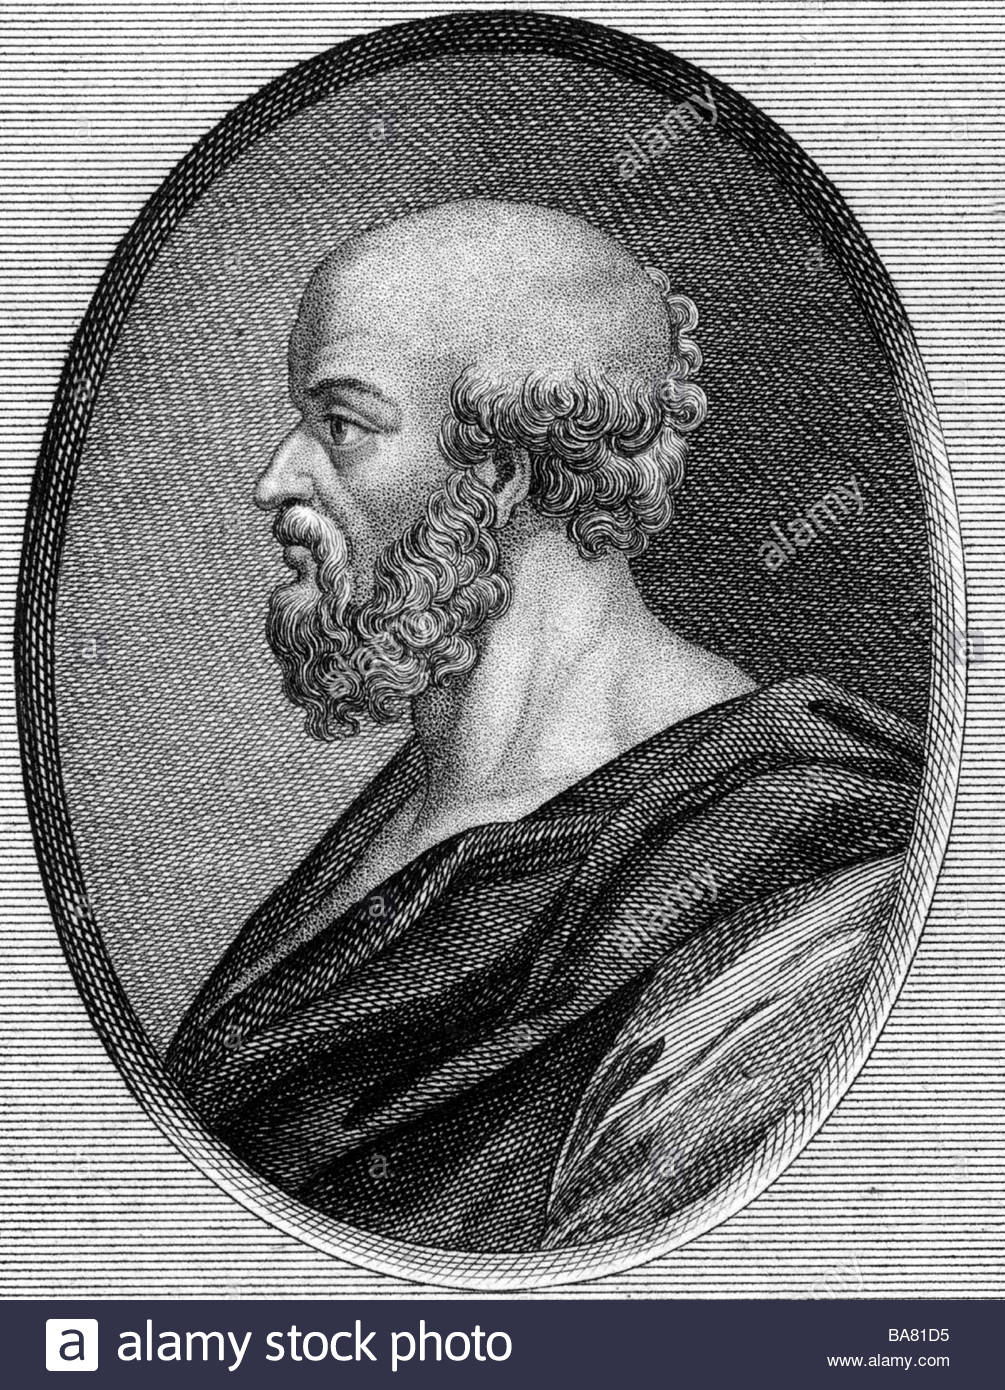
\includegraphics[scale=.1]{IMG/eratosthanes.jpg}
\end{figure}
\end{column}
\end{columns}
\end{frame}

\begin{frame}
\frametitle{The Sieve of Eratosthenes}

To find all of the prime numbers from $1$ up to some integer $n$, carry out the following:
\begin{enumerate}[(1)]
\item Write a list of all integers from 2 through $n$.
\item Start with $p=2$, the smallest prime.
\item Cross out every multiple of two in the list.
\item Return to the first uncrossed number in your list. Cross out all of its multiples.
\item Repeat until you reach the end of the list.
\end{enumerate}
\end{frame}


\begin{frame}
\frametitle{Infinity of Primes}

\begin{columns}
\begin{column}{0.5\textwidth}
What is widely regarded as one of the most beautiful proofs in history was written by the Greek mathematician Euclid, showing that there are an infinite number of primes. \newline

It uses a method called \textbf{reductio ad absurdum} or \textbf{proof by contradiction}, where you assume the negation of your conclusion is true and show that then some portion of your premise must be false. 
\end{column}
\begin{column}{0.5\textwidth}
\begin{figure}
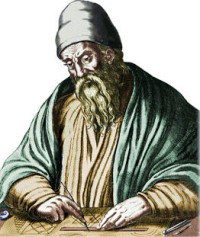
\includegraphics[scale=.5]{IMG/euclid.jpg}
\end{figure}
\end{column}
\end{columns}
\end{frame}

\begin{frame}
\frametitle{Infinity of Primes}

\begin{theorem}[Euclid]
There are infinitely many prime numbers. 
\end{theorem}
\begin{proof}
Assume to the contrary that there are only a finite number of primes. Because the list of prime numbers is finite, they are enumerable, meaning we can list them. Say that 
\[
p_1, p_2, \dots, p_k
\]
constitutes a complete list of prime numbers. \newline

\emph{Continued on next slide.}
\end{proof}
\end{frame}

\begin{frame}
\frametitle{Infinity of Primes}

\begin{proof}
\emph{Continued.}

Consider the number
\[
n = p_1p_2\cdots p_k + 1.
\]
This number cannot be prime, due to our assumption that we have already listed all of the primes. Let $d$ be the smallest divisor of $n$ which is not $1$. None of the primes in our list can be equal to $d$, because $n$ divided by $p_i$ has a remainder of $1$ for any $1\le i \le k$. Therefore, $d$ must be a prime value greater than $p_k$, a contradiction.
\end{proof}
\end{frame}


\begin{frame}
\frametitle{Prime Modulus Arithemetic}

Computing values modulo some prime $p$ is the the main application of prime numbers in cryptography. We compute values \textbf{modulo some prime $p$} if we use  only the numbers
\[
0, 1, 2, \dots, p-1.
\]
Perform all computations as you normally would, then \textbf{reduce} your answer modulo $p$, denoted $\pmod p$.
\end{frame}

\begin{frame}
\frametitle{Modular Arithmetic}

For example,
\[
(25 \mod 7) = 4.
\]
When you divide $25$ by $7$, you end up with a multiple of $4$, which is its value reduced modulo $7$. You can also compute modular reductions by adding/subtracting multiples of the modulus:
\[
25 = 25 - 21 = 4 \pmod 7
\]
\[
100 = 100 - 70 = 30 = 30 - 28 = 2 \pmod 7
\]
\[
-5 = -5 + 17 = 12 \pmod{17}
\]
Note that our final answer must always be a positive value $x$ where $0 \le x < p$.
\end{frame}

\begin{frame}
\frametitle{Multiplication}

Multiplication is carried out similarly; first multiply as you normally would, then reduce modulo $p$.
\begin{itemize}
\item $(5\cdot 3 \mod 7) = 1$
\item $6\cdot 9 = 54 = 54 - 43 = 11 \pmod{43}$
\item $5\cdot(-2) = -10 = -10 + 17 = 7\pmod{17}$
\item $((-7)\cdot 3 \mod{19}) = 17$
\end{itemize}
\end{frame}

\begin{frame}
\frametitle{Multiplication}

\begin{theorem}
For any prime $p$, $(p-1)^2 = 1\pmod p$.
\end{theorem}
\begin{proof}
Observe:
\begin{align*}
(p-1)^2 &= p^2 -2p + 1 \pmod p\\
	&= 1 \pmod p
\end{align*}
\end{proof}
\end{frame}


\begin{frame}
\frametitle{Exponentiation}

We exponentiate again by computing as we regularly would, then reducing modulo $p$.
\begin{itemize}
\item $4^6 = 4096 = 1 \pmod 7$
\item $19^{96} = 1 \pmod{97}$
\item $8292^8 = 1 \pmod 9$
\end{itemize}
Are we noticing a pattern?
\end{frame}

\begin{frame}
\frametitle{Fermat's Little Theorem}

Fermat's Little Theorem makes reduction of exponents modulo a prime much more quick.

\begin{theorem}
For a prime value $p$ and any integer $a$, 
\[
a^{p-1} = 1 \pmod p.
\]
Equivalently,
\[
a^p = a \pmod p.
\]
\end{theorem}
\end{frame}

\begin{frame}
\frametitle{Fermat's Little Theorem}

For example, say we wish to compute $(2^{1939} \mod{89})$. Observe that $1939 = (22)(88) + 3$. Therefore, 
\begin{align*}
2^{1939} \mod{89} &= 2^{(22)(88) + 3} \\
	&= (2^{22})^{88}\cdot 2^{3} \\
	&= 2^{3} \\
	&= 8\pmod{89}
\end{align*}
\end{frame}



\begin{frame}
\frametitle{Useful Tips For Computations Modulo p}

\begin{itemize}
\item You can add/subtract any multiple of $p$ from your number.
\item Results should always lie within the range $0, 1, \dots, p-1$.
\item Any value raised to the $(p-1)$th power reduces to $1$ modulo $p$.
\end{itemize}
\end{frame}


\begin{frame}
\frametitle{Groups and Finite Fields}

Mathematicians call the set of numbers modulo a prime p a \textbf{finite field} and
often refer to it as the ``mod p'' field. Different notations for this field you might encounter include $\mathbb{Z}_p$, $\mathrm{GF}(p)$, or $\mathbb{Z}/p\mathbb{Z}$.\newline 

The branch of mathematics called \textbf{abstract algebra} has large areas devoted to the study of prime fields.
\end{frame}


\begin{frame}
\frametitle{Groups}

A \textbf{group} is a mathematical structure consisting of a set of numbers together with some binary operation. A group is \textbf{closed under addition}, contains an \textbf{identity} element, and every element has an \textbf{inverse}. \newline

\textbf{Group theory} is another wide and important branch of abstract algebra. This class requires only some very basic introductory group theory.
\end{frame}

\begin{frame}
\frametitle{Additive Group Modulo p}

In this class, we do not need to make this too complicated! We consider the group $\mathbb{Z}_p$, which is the set of numbers $0, 1, 2, \dots, p-1$, together with addition. Denote this group $(\mathbb{Z}_p, +)$, the \textbf{additive group modulo p}.\newline

In the additive case we could also consider a group $(Z_n, +)$, where $n$ is a composite modulus.
\end{frame}

\begin{frame}
\frametitle{The Group $\mathbb{Z}_p$}

Let's verify the group properties for $\Z_p$, also denoted $(\mathbb{Z}_p, +)$.
\begin{itemize}
\item \emph{Closed under addition?} Adding any two elements in $\Z_p$ and reducing modulo $p$ yields an element in $\Z_p$. Therefore, $\Z_p$ is \textbf{closed under addition.}
\item \emph{Contains identity?} The \textbf{identity element} in $(\Z_p, +)$ is $0$. This means that for any $a$ in $\Z_p$, we have that 
\[a + 0 = 0+ a = a\pmod p.\]
\item {\emph{Contains inverses?}} The \textbf{inverse} of an element $a$ in $(\Z_p, +)$ is $(-a \mod p)$. This means that:
\[
a + (-a) = (-a) + a = 0 \pmod p.
\]
\end{itemize}
\end{frame}

\begin{frame}
\frametitle{Multiplicative Group Modulo p}

The \textbf{multiplicative group modulo $p$} is denoted $\Z_p^*$. This is the group composed of the set of numbers $1, 2, \dots, p-1$ with the operation of addition modulo $p$. Note that $0$ is not included here. \newline

Note that $Z_p^*$ is a group if and only if $p$ is prime.
\end{frame}

\begin{frame}
\frametitle{The Group $(\mathbb{Z}_p, +)$}

Let's verify that $\Z_p^*$ is a group.
\begin{itemize}
\item \emph{Closed under addition?} Multiplying any two elements in $\Z_p^*$ and reducing modulo $p$ yields an element in $\Z_p^*$. Therefore, $\Z_p^*$ is \textbf{closed under multiplication.}
\item \emph{Contains identity?} The \textbf{identity element} in $\Z_p^*$ is $1$. This means that for any $a$ in $\Z_p^*$, we have that 
\[a\cdot 1 = 1\cdot a = a\pmod p.\]
\item {\emph{Contains inverses?}} The \textbf{inverse} of an element $a$ in $\Z_p^*$ is some value $b$ such that This means that:
\[
ab = ba = 1 \pmod p.
\]
Some number $b$ satisfying this property always exists when $p$ is prime; we skip the proof of this for now.
\end{itemize}
\end{frame}


\begin{frame}
\frametitle{Subgroups}

A \textbf{subgroup} of a group consists of some subset of elements from the group which form a group themselves.
\end{frame}

\begin{frame}
\frametitle{Subgroups Examples}

Consider the group $(\Z_8, +)$. This group contains several subgroups. Subgroups include $\Z_2$ and $\Z_4$. \newline

This group has a subgroup consisting of the elements $\{0, 4\}$ under addition, as well as the subgroup consisting of the elements $\{0, 2, 4, 6\}$ under addition. How can we convince ourselves that these are subgroups?
\end{frame}

\begin{frame}
\frametitle{Subgroups Examples}

The multiplicative group $\Z_p^*$ has subgroups as well. Consider $\Z_7^*$ which consists of $\{1, 2, 3, 4, 5, 6\}$ under multiplication. Subgroups include:
\begin{itemize}
\item $\{1,6\}$ 
\item $\{1, 2, 4\}$
\end{itemize}
How can we check that these are, in fact, subgroups? Does $\{1, 5\}$ form a subgroup under multiplication modulo $7$? Why or why not?
\end{frame}


\begin{frame}
\frametitle{Subgroups in Cryptography}

Many cryptographic protocols make use of subgroups. We've discussed addition, subtraction, multiplication, and exponentiation modulo $n$.\newline

The two remaining properties we must discuss are \textbf{division} and \textbf{logarithms} modulo $n$.
\end{frame}


\begin{frame}
\frametitle{Division: The GCD Algorithm}

The \textbf{greatest common divisor (GCD)} of two numbers $a$ and $b$ is the largest value $k$ such that $k|a$ and $k|b$. This is often denoted $(a,b) = k$.\newline

For example, the GCD of $24$ and $30$ is $6$, also written $(24, 30) = 6$.
\end{frame}




\begin{frame}
\frametitle{Division: The GCD Algorithm}

Euclid wrote an algorithm which computes the GCD of two numbers. This algorithm is still used today and has important applications in cryptography.
\end{frame}


\begin{frame}
\frametitle{The GCD Algorithm}

Say we wish to find the GCD of $12$ and $45$. Observe that $45 = 9 \pmod{12}$. Therefore, we can write out:
\begin{align*}
45 &= 3 \cdot 12 + 9
\end{align*}
Next we compute $9 \pmod{12}$.
\begin{align*}
12 &= 1 \cdot 9 + {\color{red}\mathbf{3}} 
\end{align*}
Lastly we see that $3 = 0 \pmod 9$, and hence we are done! We have found the GCD, 3.
\end{frame}

\begin{frame}
\frametitle{The GCD Algorithm}

Next let's find the GCD of $1512$ and $784$.
\begin{align*}
1512 &= 1 \cdot 784 + 728 \\
784 &= 1 \cdot 728 + {\color{red}\mathbf{56}} \\
728 &= 13\cdot 56
\end{align*}
\end{frame}


\begin{frame}
\frametitle{The GCD Algorithm}

Now let's find the GCD of $270$ an $192$.
\begin{align*}
270 &= 1\cdot 192 + 78\\
192 &= 2\cdot 78 + 36\\
78 &= 2\cdot 36 + {\color{red}\mathbf{6}}\\
36 &= 6\cdot 6
\end{align*}
\end{frame}


\begin{frame}
\frametitle{The GCD Algorithm}

\textbf{Input:} Positive integers $a$ and $b$.

\textbf{Output:} $k$, where $(a, b) = k$.

\begin{enumerate}[(1)]
\item  While $a \ne 0$:
	\begin{itemize}
	\item $(a,b) \leftarrow (b\pmod a, a)$
	\end{itemize}
\item Return $b$.
\end{enumerate}
\end{frame}


\begin{frame}
\frametitle{The GCD Algoirthm}

For example, say our inputs are $24$ and $30$. The algorithm runs as follows:
\begin{enumerate}[Loop 1:]
\setcounter{enumi}{-1}
\item $(a, b) = (24, 30)$
\item $(a, b) = (6, 24)$
\item $(a, b) = (0, 6)$
\end{enumerate}
And the algorithm returns $6$.
\end{frame}


\begin{frame}
\frametitle{The GCD Algoirthm}

For example, say our inputs are $12$ and $45$. The algorithm runs as follows:
\begin{enumerate}[Loop 1:]
\setcounter{enumi}{-1}
\item $(a, b) = (12, 45)$
\item $(a, b) = (9, 12)$
\item $(a, b) = (3, 9)$
\item $(a, b) = (0, 3)$
\end{enumerate}
And the algorithm returns $3$.
\end{frame}

\begin{frame}
\frametitle{Coding Exercises: Euclid's GCD Algorithm}

Write Python code which carries out Euclid's GCD algorithm. 
\end{frame}


\begin{frame}
\frametitle{Least Common Multiples}

The \textbf{Least Common Multiple (LCM)} of two numbers is the smallest number that is a multiple of both of them. Find the LCM of $a$ and $b$ with the following formula:
\[
\mathrm{LCM}(a,b) = \frac{ab}{(a,b)}
\]
\end{frame}


\begin{frame}
\frametitle{Division Modulo $p$}

Euclid's algorithm provides us with the GCD of two numbers, but this is not \emph{quite} enough for division modulo $p$. \newline

What else do we need?
\end{frame}


\begin{frame}
\frametitle{Division Modulo $p$}

While computing $(a,b) = d$, we also need to find integers which allow us to express $d$ as a \textbf{linear combination} of $a$ and $b$. In other words, we need integers $r$ and $s$ such that 
\[
d = as + br
\]
How does \emph{this} help us?
\end{frame}

\begin{frame}
\frametitle{Division Modulo $p$}

When we say we want to divide modulo $p$, what we want to do is compute the value 
\[
\frac{1}{b}  \pmod p.
\]
also called the \textbf{inverse} of $b$ modulo $p$. 
\end{frame}


\begin{frame}
\frametitle{Division Modulo $p$}

We know that $p$ is prime, and $b$ is some value between $1$ and $p-1$.\newline

What is the GCD of $p$ and $b$?
\[
(a,b) = ?
\]
\end{frame}

\begin{frame}
\frametitle{Division Modulo $p$}

The GCD of a prime $p$ and a positive integer $b$, $0<b\le p-1$, is always going to be
\[
(b,p) = 1.
\]
Amazing!
\end{frame}


\begin{frame}
\frametitle{Division Modulo $p$}

Any two numbers can be written as a linear combination of their GCD. Since the GCD of $b$ and $p$ is $1$, we can find values $r$ and $s$ such that
\[
1 = br + ps.
\]
If we take this modulo $p$, we have that
\[
1 = br + ps \pmod p.
\]
\end{frame}

\begin{frame}
\frametitle{Division Modulo $p$}

We have
\[
1 = br + ps \pmod p.
\]
Let's reduce this! Since $p = 0 \pmod p$, we have:
\[
1 = br \pmod p.
\]
Ultimately for us, this means we have found the inverse of $b$ modulo $p$! Specifically, 
\[
\frac{1}{b} = r \pmod p.
\]
\textbf{WOW!}
\end{frame}


\begin{frame}
\frametitle{Division Modulo $p$}

We see in order to divide modulo a prime $p$, we need to be able to express $(p,b) = 1$ as a linear combination of $p$ and $b$.
\end{frame}


\begin{frame}
\frametitle{Euclid's Algorithm, But Backwards}

Let's use Euclid's algorithm to express $3$ as a linear combination of $12$ and $45$. First, we will carry out Euclid's algorithm. Let's use the example from a previous slide of $270$ an $192$.
\begin{align*}
270 &= 1\cdot 192 + 78\\
192 &= 2\cdot 78 + 36\\
78 &= 2\cdot 36 + {\color{red}\mathbf{6}}\\
36 &= 6\cdot 6
\end{align*}
We now want to re-write this \textbf{backwards} in order to express $6$ as a linear combination of $270$ and $192$.
\end{frame}

\begin{frame}
\frametitle{Euclid's Algorithm, But Backwards}
Let's go backwards through the computations above. On the right, let's re-write the remainder at each step as a linear combination.
\begin{align*}36 &= 6\cdot 6 & & \\
78 &= 2\cdot 36 + {\color{red}\mathbf{6}}&  6 &= 78 - 2\cdot 36 \\
192 &= 2\cdot 78 + 36 &  &= 78 - 2(192 - 2\cdot 78)\\
 & & &= 5\cdot 78 - 2 \cdot 192 \\
270 &= 1\cdot 192 + 78 &  &= 5(270 - 192) -2(192) \\
&  & & = 5\cdot 270 - 7\cdot 192
\end{align*}
\end{frame}

\begin{frame}
\frametitle{Euclid's Algorithm, But Backwards}

We did it!

\[
6 = 5\cdot 270 + (-7)\cdot 192
\]

Amazing. Now, let's automate this entire process with \textbf{Euclid's Extended Algorithm}.
\end{frame}


\begin{frame}
\frametitle{Euclid's Extended Algorithm}

\textbf{Input:} Non-negative integers $a$ and $b$.

\textbf{Output:} $d$, where $(a, b) = d$, as well as integers $r$ and $s$ such that $d = ar + bs$.

\begin{enumerate}[(1)]
\item $(c,d) \leftarrow (a,b)$
\item $(u_c, v_c, u_d, v_d) \leftarrow (1, 0, 0, 1)$
\item  While $c \ne 0$:
	\begin{itemize}
	\item $q \leftarrow [d/c]$
	\item $(c,d) \leftarrow (d-qc, c)$
	\item $(u_c, v_c, u_d, v_d) \leftarrow (u_d - qu_c, v_d-qv_c, u_c, v_c)$
	\end{itemize}
\item Return $d, (u_d, v_d)$
\end{enumerate}
\end{frame}


\begin{frame}
\frametitle{Example: Euclid's Extended Algorithm}

For our first example let's look at $270$ and $192$ again.
\begin{enumerate}[(1)]
\item $(c,d) \leftarrow (192, 270)$
\item $(u_c, v_c, u_d, v_d) = (1, 0, 0, 1)$
\item  \begin{enumerate}[(Round 1)]
 \item           
          \begin{itemize}
          \item $q \leftarrow [270/192] = 1$
          \item $(c,d) \leftarrow (270-1\cdot 192, 192) = (78, 192)$
          \item $(u_c, v_c, u_d, v_d) = (-1, 1, 1, 0)$
          \end{itemize}
 \item 
          \begin{itemize}
          \item $q \leftarrow [192/78] = 2$
          \item $(c,d) \leftarrow (192 - 2\cdot 78, 78)  = (36, 78)$
          \item $(u_c, v_c, u_d, v_d) \leftarrow (3, -2, -1, 1)$
          \end{itemize}
  \item
  		\begin{itemize}
          \item $q \leftarrow [78/36] = 2$
          \item $(c,d) \leftarrow (78-2\cdot 36, 36) = (6,36)$
          \item $(u_c, v_c, u_d, v_d) \leftarrow (-7, 5, 3, -2)$
  		\end{itemize}
  \item 
         \begin{itemize}
          \item $q \leftarrow [36/6] = 0$
          \item $(c,d) \leftarrow (78-2\cdot 36, 36) = (0,6)$
          \item $(u_c, v_c, u_d, v_d) \leftarrow (17, -12, -7, 5)$
  		\end{itemize}
\end{enumerate}
\item Return $d=6$ and $(u_d, v_d) = (-7, 5)$
\end{enumerate}
\end{frame}

\begin{frame}
\frametitle{Example: Euclid's Extended Algorithm}

We see that input $(192, 270)$ yield outputs $d=6$ and $(u_d, v_d) = (-5, 3)$. This means that
\[
6 = (-7)\cdot 192 + (5) \cdot 270
\]
\end{frame}



\begin{frame}[fragile]
\frametitle{Working Modulo 2}

While not of specific interest in this class, group theory has applications in computer science beyond cryptography. Addition and multiplication modulo the prime $2$ are equivalent to the \verb|XOR| and \verb|AND| gates, respectively. \newline


\begin{columns}
\begin{column}{.3\textwidth}
\begin{tabular}{ r|c|c| }
\multicolumn{1}{r}{}
 &  \multicolumn{1}{c}{0}
 & \multicolumn{1}{c}{1} \\
\cline{2-3}
0 &  0&  1\\
\cline{2-3}
1 & 1&0 \\
\cline{2-3}
\end{tabular}\newline

\verb|    XOR|\newline add. $\pmod 2$
\end{column}

\begin{column}{.3\textwidth}
\begin{tabular}{ r|c|c| }
\multicolumn{1}{r}{}
 &  \multicolumn{1}{c}{0}
 & \multicolumn{1}{c}{1} \\
\cline{2-3}
0 &  0&  1\\
\cline{2-3}
1 &1 & 1\\
\cline{2-3}
\end{tabular}\newline

\verb|    AND|\newline mult. $\pmod 2$
\end{column}
\end{columns}
\end{frame}



\begin{frame}[fragile]
\frametitle{Large Primes: C/C++}

Cryptographic protocols often use \textbf{large primes} which are hundreds of digits long. In programming languages like C++ this means we need \textbf{multiple precision libraries} because the \verb|int| and \verb|long int| data types do not allocate enough storage for numbers as large as these primes, and even the \verb|float| type does not yield the required precision. \newline

One such library for Cis called \textbf{GMP}, the GNU Multiple Precision Arithmetic Library. You can download and read about its implementation here:
\begin{center}
\url{https://gmplib.org/}
\end{center}
\end{frame}

\begin{frame}[fragile]
\frametitle{Large Primes: Python}

Storage allocation works very differently in Python from most programming languages. You do not need to specify memory allocation up front. This gives an ease of use and flexibility other programming languages lack. \newline

However, when working with such large numbers, it often becomes necessary to control memory allocation very precisely. C++ is often used in cryptography for this reason. However it will be sufficient for us to use Python for the scope of this course. 
\end{frame}



\begin{frame}[fragile]
\frametitle{Large Primes: Python}

Since data types in Python are not limited to a certain number of bits, to determine the maximum integer size we simply see how many bits of memory the computer holds. \newline

We can use the \verb|sys| module to check this. For instance, on my \verb|64|-bit machine:
\begin{verbatim}
>>> import sys
>>> sys.maxsize
9223372036854775807
\end{verbatim}

This number is precisely equal to $2^{63}-1$. (On a \verb|32|-bit machine the maximum value would be $2^{31}-1$).
\end{frame}

\begin{frame}[fragile]
\frametitle{Large Primes: Python}

Thus we see that in Python on a \verb|64|-bit machine, we can store integer values up to \verb|9223372036854775807| bits long. In public-key cryptography we wish to generate primes which are only \verb|2000| to \verb|4000| bits long. Thus we do not need to use a multiple precision library in Python to work with large primes. 
\end{frame}


\begin{frame}
\frametitle{Generating Large Primes}

How do we generate a large prime? Any ideas?
\end{frame}


\begin{frame}
\frametitle{Generating Large Primes}

To generate a large prime $p$ in the neighborhood of some large number $n$, we simply 
\begin{enumerate}[Step 1:]
\item Pick a random value $p$ in the ``neighborhood'' of $n$
\item Determine whether this value is random or not.
\item Repeat until $p$ is prime. 
\end{enumerate}

There are very good available algorithms for determining whether a number is prime or not. What algorithm have we looked at for determining this?
\end{frame}


\begin{frame}[fragile]
\frametitle{Generating Large Primes}

How many times will we have to repeat the loop? Perhaps surprisingly, prime numbers are actually relatively common. In the neighborhood of a number $n$ there are approximately $\ln n$ prime values! \newline

Furthermore, primality checking is often trivial -- so primality checking is very quick for many numbers. For instance, any multiple of $2$ is obviously not prime. 
\end{frame}

\begin{frame}
\frametitle{Generating Large Primes}

Primality testing is often carried out as follows:
\begin{itemize}
\item First, pick a random number $p$ in the neighborhood of $n$. 
\item Check whether $p$ is divisible by any numbers in some ``small'' range -- say, verify that $n$ has no divisors between $2$ and $1000$.
\item If $p$ has no divisors in this small range run a more ``expensive'' primality test such as the Rabin-Miller test.
\item Repeat until $p$ is prime. 
\end{itemize}
\end{frame}

\begin{frame}[fragile]
\frametitle{Generating Large Primes: Example}

Say, for instance, that we wish to find a random prime which is \verb|2000| bits long. A number of this size lies inside the range $2^{1999}$ and $2^{2000}$. We expect about $\ln(2^{1999})$ primes in this range. In fact, about one in every $1386$ numbers is prime in this range. 
\end{frame}


\begin{frame}
\frametitle{Your Next Midterm}

Midterm 2 will be partially answers to written questions which you complete individually, and partially a group coding project where you write programs for generating large primes.\newline

Next week you will receive all instructions for the second midterm including psedudocode 
\end{frame}




\begin{frame}
\frametitle{References}

\begin{itemize}
\item \emph{Cryptography Engineering} by Schneier, Ferguson, Kohno, Chapter 10
\end{itemize}
\end{frame}
\end{document}


